\documentclass[12pt, oneside]{article}
\usepackage{geometry}
\geometry{letterpaper}
\usepackage{graphicx}
\usepackage{amssymb}


\title{ExaWind FY17 Q2 Deliverable - Stand-up Code Repository and Software Build System and Test Harness}
\author{ExaWind Project Team}
\date{March 30, 2017}

\begin{document}
\maketitle

\section{Milestone Definitions}

\noindent This milestone is defined as such:

\begin{itemize}
	\item Create draft software design document, including code requirements around building, testing, and documentation.	
	\item Establish a public-facing code repository.
        \item Choose and implement build system and testing harness on dedicated testing cluster for nightly building and testing.
\end{itemize}

\noindent The milestone completion criteria is listed as such:

\begin{itemize}
	\item Software build system and test harness will be released on the project software repository, along with necessary documentation.
\end{itemize}

\section{Build and Test System Requirements}

\subsection{Build System}
The build system should ideally possess these qualities:
\begin{itemize}
	\item The ability to \textit{mostly} automate the software build process of Nalu
	\item The ability to automatically resolve and build the software dependency chain of Nalu
	\item Simplicity in the mechanism for encoding build instructions into the system
	\item Portability for building on all relevant DOE supercomputers and developer machines, for Linux, Unix, and Mac operating systems
	\item Actively developed and supported
	\item A community involving other stakeholders in the tool
	\item Ability to build with multiple compilers, manage multiple build configurations, and keep the software stack up-to-date
\end{itemize}

\section{CMake for Cross-Platform Software Building}
For Nalu's direct build system, CMake has been chosen for several reasons that support the list above. CMake is already used in many of the other software distributions Nalu relies upon. CMake promotes portability and simplicity in developing the build process for a single application. It has a solid history and is actively developed and supported, with a large community of users, which make it easy to find solutions when necessary during development. Also, many of the project developers have previous experience with CMake.

\section{Spack for Software Build Management}
For the overarching build management system, Spack has been chosen. It is a suitable package manager for this project as it possesses the qualities listed above with good support for CMake. Spack is the Supercomputing Package Manager developed at LLNL and itself is also part of the Exascale Computing Project. Commitments at some level to using Spack for application management have been made at almost every DOE lab involved in scientific and high performance computing. Notability ORNL, LLNL, NERSC, LANL, and ANL are implementing it on their largest machines. Spack has been under development for a few years now and has matured to the point that it now has dedicated developers and is becoming \textit{the} package manager to use when compared to similar projects such as EasyBuild, Smithy, SWTools, and maali (cite these), though EasyBuild is its closest competitor in both functionality and marketshare. Spack is explicitly designed with the idea that scientific software developers and users should be provided a simpler way in which they can build, manage, and run the software they rely on or develop for their research. Spack allows for building and managing software with the awareness that users requiring the highest performance possible for their applications will want to build with multiple compilers, automatically resolve and build any software dependencies, manage multiple configurations of several software stacks, keep all the software and their dependencies up-to-date, or decide to use specific versions of applications, and do all of this portably across multiple machines. In the past, this was mostly done manually, which has never been efficient, lacked the ability to quickly test different configurations of the software stacks, but most importantly is likely not sustainable in the future due to increasing complexities.

The software being developed for this project, Nalu, is a perfect case in which the building of it and its software dependencies can and should be automated using Spack, with the idea that Nalu's destiny is to be built and run now and in the future on the largest machines at the Leadership Computing Facilities as well as many other DOE machines along the way. For all these reasons, Spack makes the most sense as the tool to assist in the building of Nalu. Figure~\ref{fig:nalu-deps} shows the entire software dependency graph for Nalu excluding the requirement of a compiler.

\begin{figure}
  \centering
    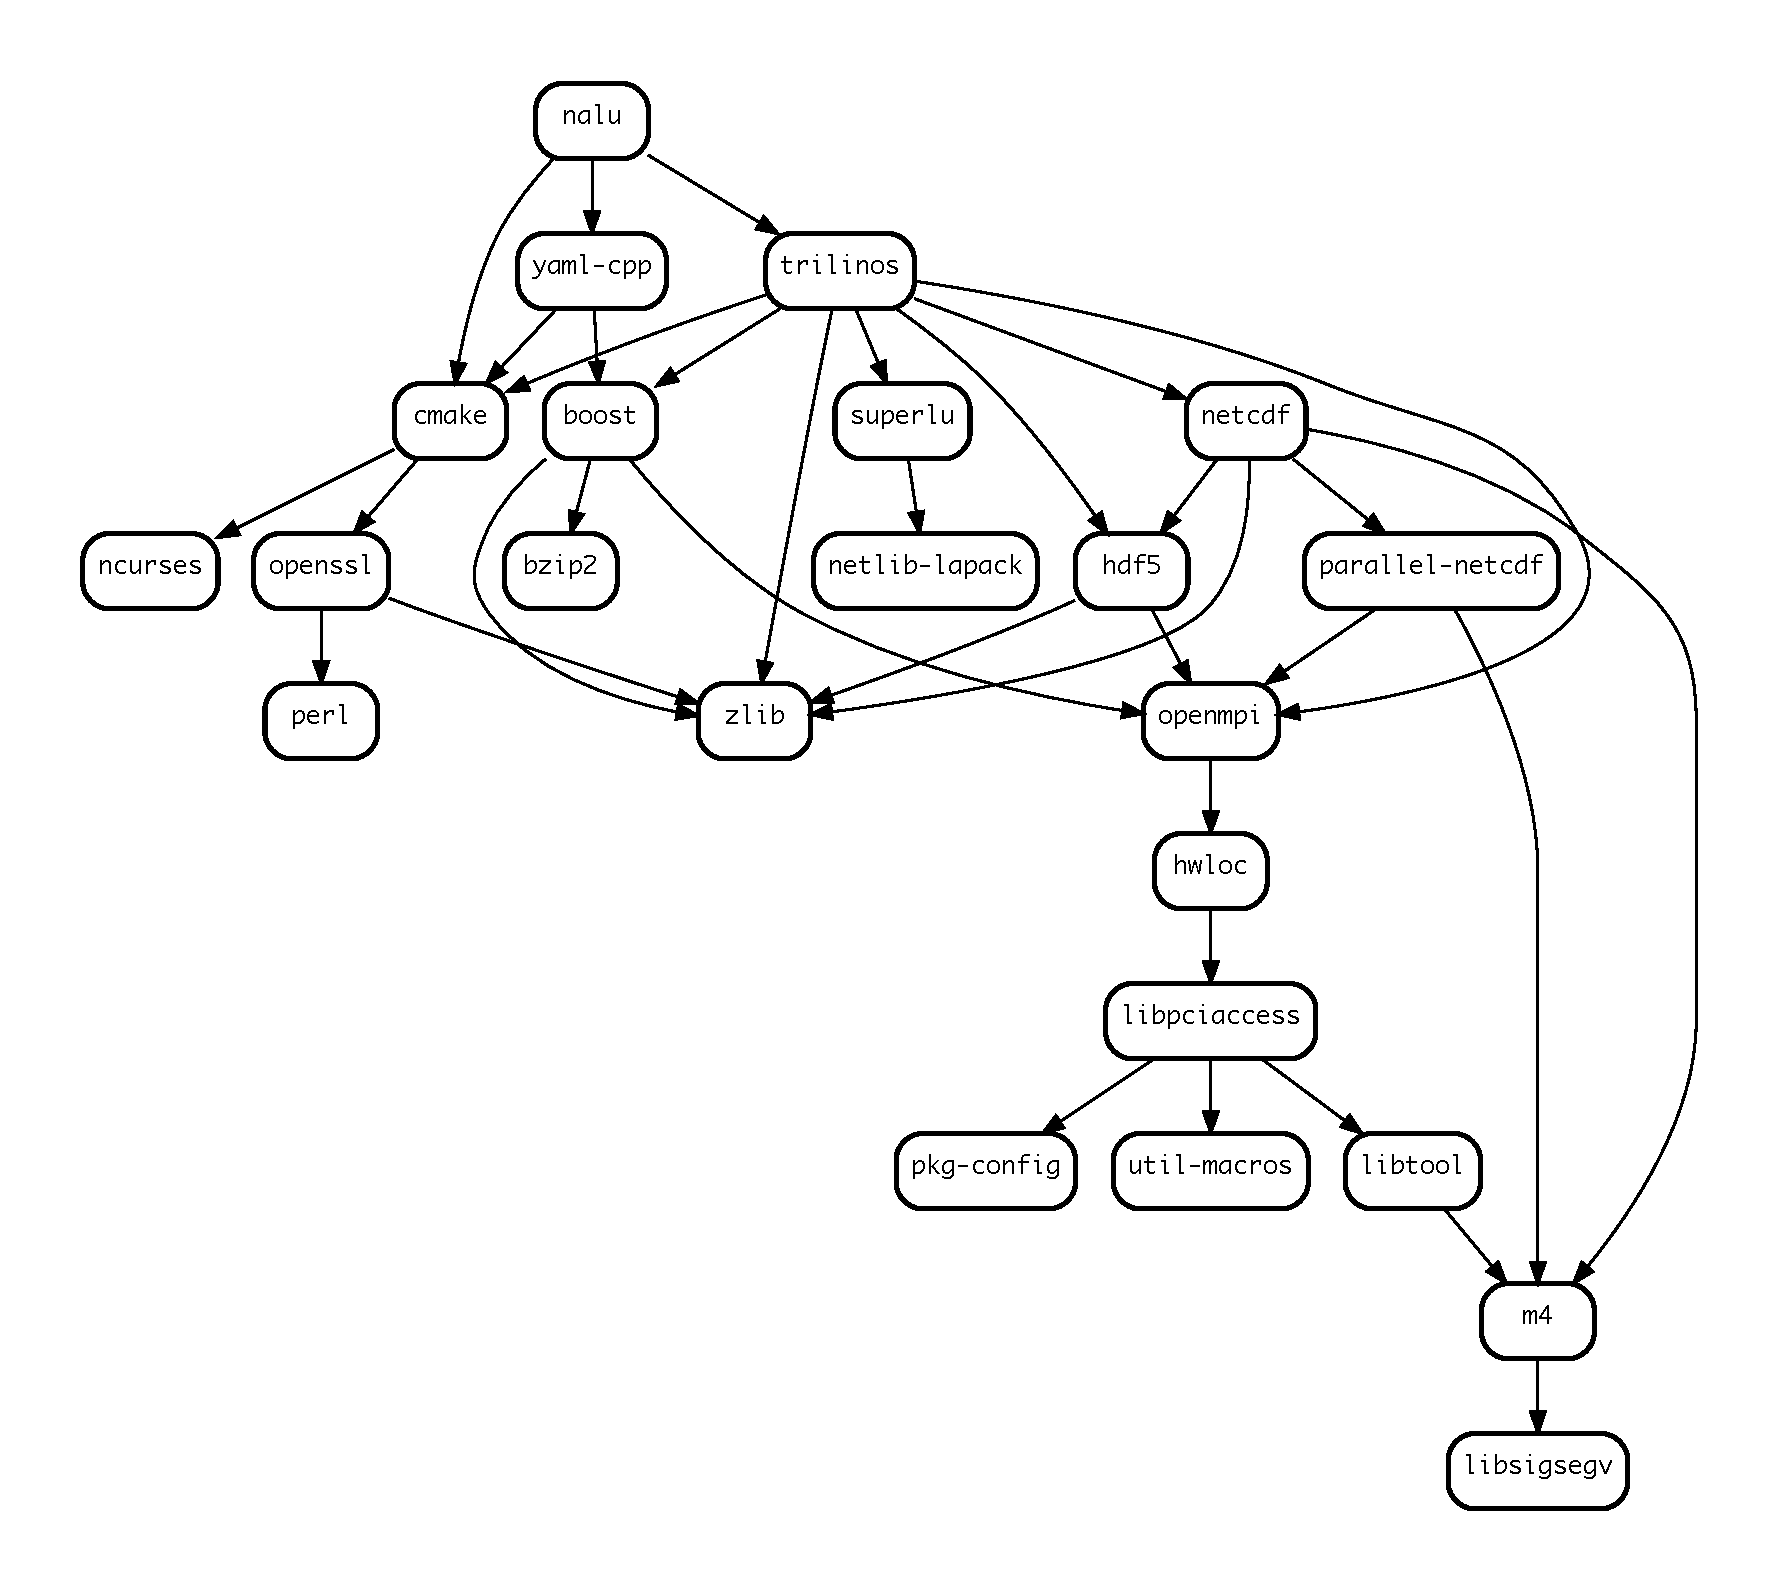
\includegraphics[width=0.6\textwidth]{nalu-graph}
  \caption{Dependency graph for Nalu.}
  \label{fig:nalu-deps}
\end{figure}

To install Nalu using Spack in theory, simply takes installing Spack and a compiler, and running the command `\texttt{spack install nalu}'. In reality, at the moment it is about a two- or three-step process after Spack is installed, depending on the machine you are on, which involves copying a Spack configuration and specifying particular versions of third-party libraries to avoid known issues with certain packages. However, we are able to build Nalu entirely using Spack and this has already been utilized to get new project members a working version of Nalu they can develop with in their own user account within a few hours.

\section{Test System}

The test system for Nalu should be able to:
\begin{itemize}
	\item Update and build Nalu
	\item Report build errors
	\item Run regression and unit tests
	\item Report test failures
	\item Execute tests on a nightly schedule
	\item Report test results to a central location easily accessible to developers for viewing
	\item Allow a developer to easily add a new test
	\item Allow a developer to easily select and run tests relevant to their work
\end{itemize}

\subsection{CTest and CDash for Testing}

For testing Nalu, CTest and CDash have been chosen as tools for accomplishing this task. CTest is a testing framework that is built into CMake and CDash is a service Kitware, the developers of CMake, provide to users of CMake in which results of tests are able to be submitted to a website, and this allows the results to be viewed easily from anywhere using a web browser.

To define a regression test, a user creates an input file for Nalu, and runs this input file to generate output. This output is then defined initially as a `gold standard' for this test. A \textit{tolerance} is then chosen that the results of the test would be able to deviate from the `gold standard' reference output and not be considered a failure of the test. Unfortunately this reference output for Nalu is not portable and must be defined on a per machine, per configuration, per compiler, per compiler optimizations, per third-party library versions, basis. Therefore, for regression testing, we must establish a single machine and configuration as our `gold standard' in which we are able to use the smallest of tolerances when deciding on test success or failure. Developers are able to run tests locally on their machines with more relaxed tolerances, but the official test machine will continue to constrain their tests to higher standards.

Fortunately running simulations in Nalu has a fairly uniform structure, so adding a new test requires the developer to simply add a line with their test name to the test list file and the amount of processors the test should use during execution. Then a list of steps necessary to prepare the test directory must be added in the CTest script for preparing the tests, which mostly involves copying input data and reference data to the test execution directory.

To keep the main Nalu source code repository lightweight, a separate repository holds the files used for testing such as meshes, input files, and reference output data. The developer is able to run the tests by checking out the Nalu regression testing repo, configuring Nalu with testing enabled, specifying the path for the regression testing repo, an empty directory where the tests will be executed, and optionally a tolerance to be used for judging test success. With Nalu compiled, the developer is able to run `\texttt{make test}' to run all of the tests, or `\texttt{ctest -R femHC}' to run a single test for example. The unit tests may also be run as part of this same framework, such as `\texttt{ctest -R unitTest1}'.

Testing for Nalu occurs nightly on a machine local to NREL. A simple testing script is run at a scheduled time each day which also utilizes Spack underneath to manage the build or rebuild or certain applications in Nalu's software stack, as well as Nalu. The testing script is somewhat portable enough, along with the power of Spack, that additional test machines in the future can be setup quickly without the overhead of organizing the software stack manually.

Results of these tests that are run nightly are submitted to the CDash website for Nalu located at `\texttt{http://my.cdash.org/index.php?project=Nalu}' and an example can be seen in Figure~\ref{fig:nalu-cdash}. Results from other machines in the future can also be easily submitted to this CDash website using the testing scripts.

\begin{figure}
  \centering
    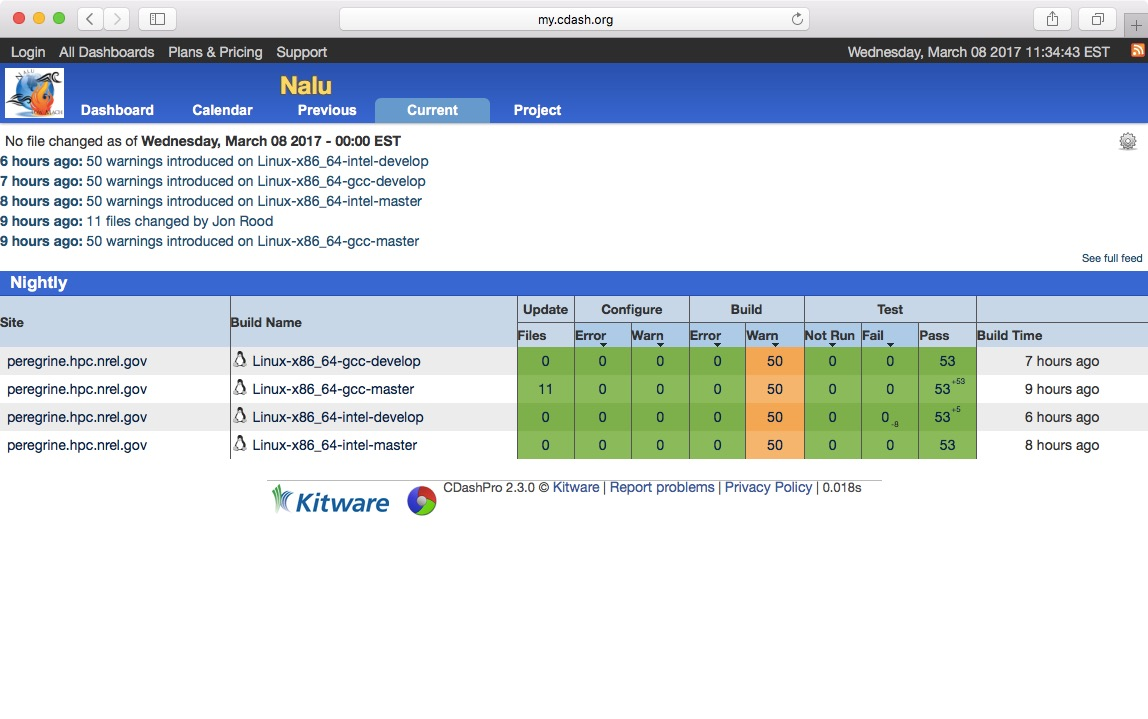
\includegraphics[width=0.8\textwidth]{nalu-cdash}
  \caption{Nalu CDash test results.}
  \label{fig:nalu-cdash}
\end{figure}

\section{Code Repository}

Github has been chosen to as the service to host and provide version control for the Nalu source code. Github is a very popular code hosting service and provides flexibility and functionality such as webhooks and integrations with many other services, as well as ability to track issues, provide metrics on development, and allow any person to make a contribution through `pull requests'. The Nalu Github website displayed in Figure~\ref{fig:nalucfd-github} is located at `\texttt{https://github.com/NaluCFD}' with the relevant repositories for the project available there regarding the source code for Nalu, testing Nalu, utilties specifically for Nalu in wind applications, LaTeX files for PDF documentation of the theory and verification manual for Nalu, a sandbox repo for testing concepts, and a repo involving building and testing of Nalu.

\begin{figure}
  \centering
    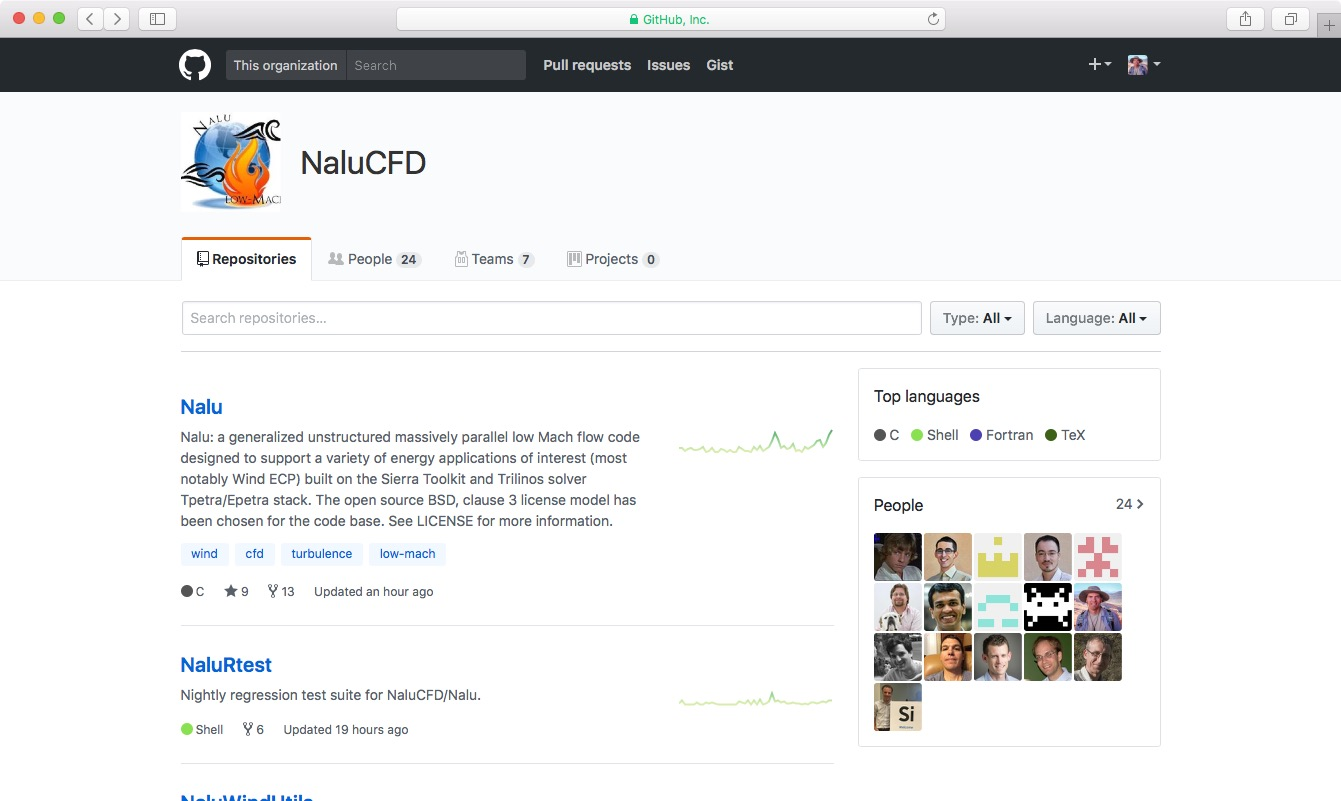
\includegraphics[width=0.8\textwidth]{nalucfd-github}
  \caption{Nalu Github organization.}
  \label{fig:nalucfd-github}
\end{figure}

\section{Project Documentation}

Documentation for Nalu in regards to this project has been designed to utilize the Sphinx, Doxygen, and Doxylink tools for generating the end-user and developer documentation. This generated documentation is then deployed to the website `\texttt{http://nalu.readthedocs.io}' automatically at each update to the Nalu Github repository. This provides up-to-date documentation for the project, which is easily accessible to everyone with a web browser as seen in Figure~\ref{fig:nalu-rtd}.

\begin{figure}
  \centering
    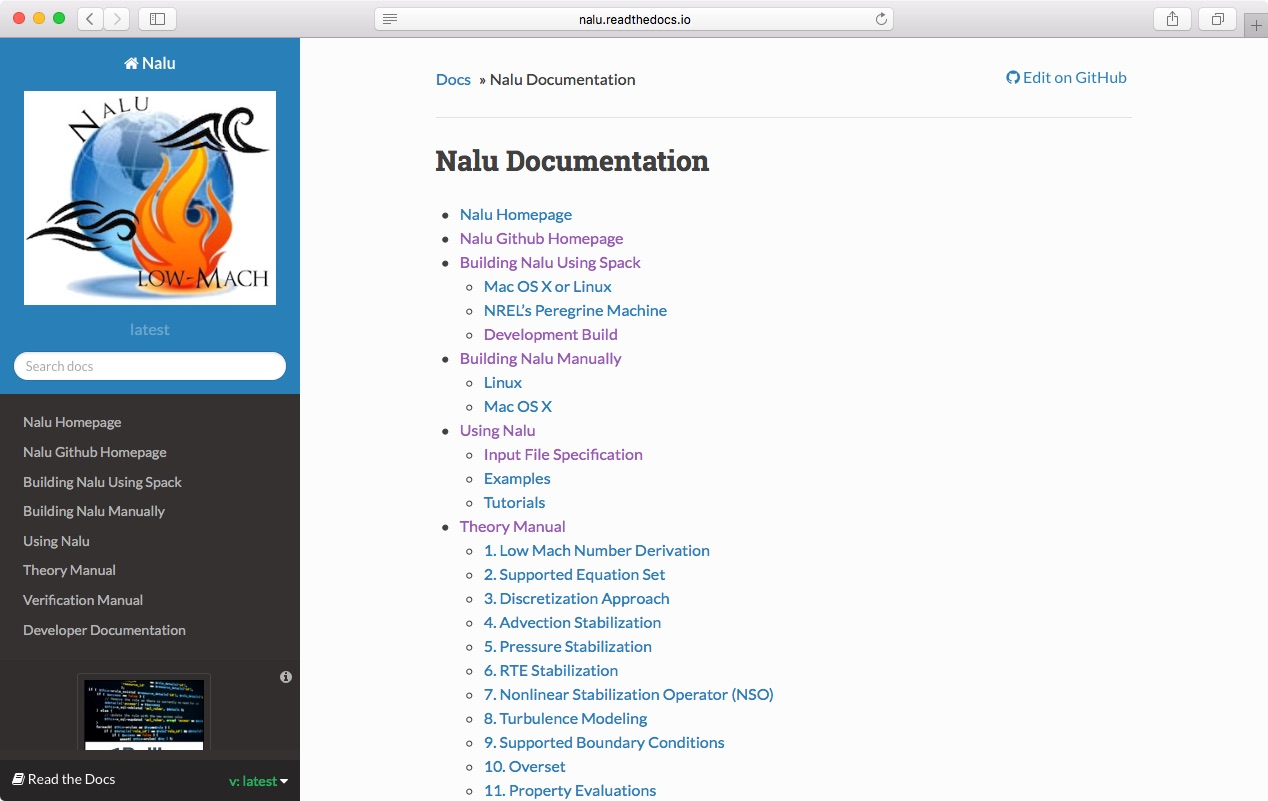
\includegraphics[width=0.8\textwidth]{nalu-rtd}
  \caption{Nalu documentation.}
  \label{fig:nalu-rtd}
\end{figure}

This documentation is developed with the ideology that two main types of users will need to read the documentation to use Nalu most effectively. These are users, and developers. With this in mind, Doxygen is used to provide a mechanism in which developers can document the code as they develop it, allowing this documentation to evolve as if it is the source code. Doxygen utilizes annotations in the code that are written as comments which are then extracted and used to generate standalone documentation about the source code. Next, Sphinx is used to create documentation that requires a more long-form human-curated approach separate from the source code itself, such as instructions on building and installing Nalu, using Nalu to run simulations, as well as developer-focused documentation such as how to document source code, how to test Nalu, etc. Doxylink allows the Sphinx documentation to reference and link to the Doxygen documentation directly. All of these tools together generate the Nalu user manual and software requirements documentation, which is then deployed to `\texttt{http://nalu.readthedocs.io}' and also able to be built locally on a user's machine.

\section{Conclusions}

A comprehensive framework for building and testing the Nalu application, which is the major focus of the ExaWind project, has been selected and implemented. The chosen framework gives focus to the project's future in simplifying the build process of our main application and making it more portable to machines it may encounter in the future. The testing framework was also able to be built on top of the build tools, which again allows for portability, functionality, and simplicity when running and creating tests in Nalu. A documentation framework was also chosen which is able to automatically generate source code documentation using annotations that live with the code, and also allows us to design and deploy user-focused and developer-focused documentation in a way that is efficient for the developer to create, and is also automatically deployed and as up-to-date as the latest source code change. This documentation framework was then utilized to create a draft of the software requirements documentation and Nalu user manual. Lastly, all of this work is hosted and available to anyone at the Github website for Nalu, `\texttt{https://github.com/NaluCFD}'.

\section{Future Work}

Future work regarding this milestone mostly involves developing the documentation around Nalu so that new users are able to effectively run simulations in Nalu, and new developers are able to effectively develop in Nalu. This will require a commitment from the project team to contribute to the documentation and consider it a requirement to development.

Although the intended dedicated machine was unable to be deployed at NREL in time for this milestone, the testing harness has been designed in such a way that it should be trivial to switch from the current machine we are testing on to this new machine when it is available.

Building Nalu using Spack currently requires a fairly customized configuration for Trilinos as Trilinos has a very large amount of options. In the future we would like to generalize this Trilinos configuration in such a way that we can then include Nalu as a package in the official Spack distribution.

The future may also involve ensuring that Nalu and its dependencies can continue to be built using Spack, and broadening this to include even more compilers than GCC and Intel. Currently we are only focusing on GCC and Intel compilers at the moment, but may want to include Clang, PGI, and Cray in the future.

We are also planning to deploy the test harness in the future inside a Docker container on our dedicated testing machine, after which we would like to distribute this container to developers for testing locally on their own machine, provided Docker can provide consistent results for the tests. This could make it easier for developers to spot deviations in the regressions tests as early as possible.

\end{document}

